\documentclass{article}

\textwidth=6.5in
\textheight=8.5in
\voffset=-54pt
\oddsidemargin=0in
\evensidemargin=0in
\setlength{\parskip}{8pt}
\setlength{\parindent}{0pt}

\usepackage{amsmath, amssymb}
\usepackage{ifthen}

\usepackage[inline]{enumitem}
\setlist{topsep=0pt, parsep=8pt}

\usepackage[rgb,table]{xcolor}\convertcolorsUfalse
\usepackage{graphicx}

% change hyperref options
\PassOptionsToPackage{hyphens}{url}
\usepackage[bookmarks,colorlinks,linkcolor=black,citecolor=blue,pdfstartview=FitH,urlcolor=blue]{hyperref}
\hypersetup{pdfpagemode=UseNone}
\usepackage{bookmark}

\usepackage{graphicx}
\usepackage{multicol}
\usepackage{framed}
\usepackage{array}

\usepackage{icomma}

\usepackage{soul}
\usepackage[normalem]{ulem}

\usepackage{pgfplots}
\pgfplotsset{compat=1.18}  
\pgfplotscreateplotcyclelist{mycolor}{black, blue, red, green!70!black, magenta, purple, cyan, orange }  
\pgfplotsset{
  disabledatascaling,
  cycle list=tikzcolor, 
  axis lines=middle,
  every axis plot/.style={no marks, thick},
  every axis/.style={
    enlarge x limits=false,
    enlarge y limits=auto,
    xlabel style={at={(current axis.right of origin)},anchor=west},
    ylabel style={at={(current axis.above origin)},anchor=south},
    % extra x and y ticks for asymptotes
    extra x tick style={grid=major, grid style={dashed,black}},
    extra y tick style={grid=major, grid style={dashed,black}},
    /pgf/number format/1000 sep={},
  },    
  tick label style = {font=\footnotesize, fill=\currentbgcolor, inner sep=0pt},    
  xticklabel shift=1pt,    
  scaled ticks=false,
  scaled y ticks=false,
  unbounded coords=jump,
  samples=101,
  minor tick length=0,
  scatter/classes={
    open={mark=*,draw=black,fill=white, mark size=2, thin},
    closed={mark=*,draw=black,fill=black, mark size=2, thin}
  },
  width=3in,
}
\pgfplotsset{open/.style={only marks, mark=*, fill=white, thin, mark size=2}}
\pgfplotsset{closed/.style={only marks, mark=*, draw=black, fill=black,
    thin, mark size=2}}
\pgfplotsset{labeled/.style={nodes near coords, only marks, mark=*, draw=black, fill=black, thin, mark size=2, point meta=explicit symbolic}}

\usepackage{tikz}
\usetikzlibrary{
  matrix,%
  % enables the snake paths
  decorations.pathmorphing,%
  % enables bigger arrows
  decorations.markings,%
  decorations.pathreplacing,%
  decorations.text,%
  calc,%
  patterns,%
  shapes.geometric,%
  arrows,
  decorations.shapes,
  positioning,
  plotmarks,
  intersections,
  tikzmark
}
\tikzset{>=latex} % sets default arrow type in tikz
\tikzset{font=\normalsize}
\tikzset{mark size=1.5pt, mark options=thin}
\tikzset{pin distance=4pt,
  every pin edge/.style={<-, thin, shorten <= -2pt}}

\interfootnotelinepenalty=10000
\renewcommand{\thefootnote}{(\arabic{footnote})}

\usepackage{multirow, bigdelim}

% change to \usepackage[sols]{handout} to see solutions
\usepackage[sols, notes]{handout}

\newcommand\iscurrentenumi[1]{%
  \ifthenelse{\equal{#1}{\theenumi}}{}{#1}}
\setenumerate[1]{ref=\#\arabic*}
\setenumerate[2]{ref=\protect\iscurrentenumi{\theenumi}(\alph*)}
\newcommand\enumiiprefix[2]{%
  \ifthenelse{{\equal{#1}{\theenumi}}\AND{\equal{#2}{(\alph{enumii})}}}{}{}%
  \ifthenelse{{\equal{#1}{\theenumi}}\AND{\NOT{\equal{#2}{(\alph{enumii})}}}}{#2}{}%
  \ifthenelse{\equal{#1}{\theenumi}}{}{#1#2}%
}
\setenumerate[3]{ref=\protect\enumiiprefix{\theenumi}{(\alph{enumii})}\roman*}

\newlength{\tipmargin}
\makeatletter

\newdimen\SOUL@dimen %new
\def\SOUL@ulunderline#1{{%
    \setbox\z@\hbox{#1}%
    % \dimen@=\wd\z@
    \SOUL@dimen=\wd\z@ %new
    \dimen@i=\SOUL@uloverlap
    \advance\SOUL@dimen2\dimen@i %\dimen@ exchanged too
    \rlap{%
      \null
      \kern-\dimen@i
      % \SOUL@ulcolor{\SOUL@ulleaders\hskip\dimen@}%
      \SOUL@ulcolor{\SOUL@ulleaders\hskip\SOUL@dimen}% new
    }%
    \unhcopy\z@
  }}
\newcommand\binomialCoefficient[2]{%
  % Store values 
  \c@pgf@counta=#1% n
  \c@pgf@countb=#2% k
  % 
  % Take advantage of symmetry if k > n - k
  \c@pgf@countc=\c@pgf@counta%
  \advance\c@pgf@countc by-\c@pgf@countb%
  \ifnum\c@pgf@countb>\c@pgf@countc%
  \c@pgf@countb=\c@pgf@countc%
  \fi%
  % 
  % Recursively compute the coefficients
  \c@pgf@countc=1% will hold the result
  \c@pgf@countd=0% counter
  \pgfmathloop% c -> c*(n-i)/(i+1) for i=0,...,k-1
  \ifnum\c@pgf@countd<\c@pgf@countb%
  \multiply\c@pgf@countc by\c@pgf@counta%
  \advance\c@pgf@counta by-1%
  \advance\c@pgf@countd by1%
  \divide\c@pgf@countc by\c@pgf@countd%
  \repeatpgfmathloop%
  \the\c@pgf@countc%
}

\renewenvironment{framed}{
  \setlength{\tipmargin}{\textwidth-\linewidth}
  \advance\@totalleftmargin-\tipmargin
  \def\FrameCommand{\hspace{\tipmargin}\fbox}%
  \advance\linewidth\tipmargin
  \MakeFramed {\advance\hsize-\width \FrameRestore}%
}
{\endMakeFramed}

\makeatother

\definecolor{purple}{rgb}{0.5,0,1.0}

\usepackage{fancyhdr}
\lhead{\textcolor{white}{This content is protected and may not be shared, uploaded, or distributed.}}
\rhead{}
\rfoot{\vspace*{\fill}\footnotesize\textcopyright{} \emph{Harvard Math Ma}}
\renewcommand{\headrulewidth}{0pt}
\pagestyle{fancy}
\begin{document}

\htitle{3 Differentiation Rules}

\begin{problemonly}
  \begin{framed}

You should be able to:
    \begin{itemize}[topsep=0pt,partopsep=0pt,parsep=8pt,itemsep=0pt]
    \item Explain why the Power Rule is true for positive integer exponents.

    \item Explain why the Constant Multiple Rule and Sum Rule are true.

    \item Use the Power Rule, Constant Multiple Rule, and Sum Rule, and recognize when they do and do not apply.

    \end{itemize}
  \end{framed}
\end{problemonly}

\begin{quote}
  {\it Civilization advances by extending the number of
    important operations which we can perform without thinking about
    them.} \\
  \hspace*{\fill} -- Alfred Whitehead, mathematician and
  philosopher\hspace*{0.5in} 
\end{quote}

\note{Here, I will try to really emphasize that the derivative of a constant is 0.}

We've previously found the derivatives of several functions; fill in the empty boxes. (You should be able to do these by thinking graphically.) Also, rewrite the last two derivatives in the form $a x^b$.

{
  \renewcommand{\arraystretch}{3}

  \begin{tabular}{|c|c|c|c|c|c|c|}
    \hline
    \textbf{Function} & \ $7$\ & \ $x$ \ & $5x + 3$ & $x^2$ & $x^{-1} =
    \dfrac{1}{x}$ & $x^{-2} = 
    \dfrac{1}{x^2}$ \\
    \hline
    \textbf{Derivative} & \solonly{0} &
    \solonly{1} & \solonly{5} &
    $2x$ & $- \dfrac{1}{x^2} = \fitb{0.5in}{- x^{-2}}$ & $- \dfrac{2}{x^3} = \fitb{0.5in}{-2x^{-3}}$ \\
    \hline
  \end{tabular}
}

\begin{enumerate}
\item  

  \begin{problem}[\stretch{0.75}]
    We'd like to find the derivative of $x^n$ where $n$ is a positive
    integer. Write out the limit definition of $\frac{d}{dx}(x^n)$.
    (In other words, if $f(x) = x^n$, write out the limit definition
    of $f'(x)$. 
  \end{problem}

\item  \emph{Exploring $(x + h)^n$.} 

  We know $(x + h)^0 = \fitb{0.25in}{1}$ and $(x + h)^1 = \fitb{0.5in}{x + h}$. Now, expand:
  \begin{enumerate}
  \item
    \begin{problem}[0.25in]
      $(x + h)^2$
    \end{problem}

    \begin{solution}
        $(x+h)^2=(x+h)(x+h)=x^2+2xh+h^2$
    \end{solution}

  \item
    \begin{problem}[\vfill\newpage]
      $(x + h)^3$ (Can you make use of what you just found out about $(x + h)^2$?)
    \end{problem}

    \begin{solution}
      \begin{align*}
        (x+h)^3 &= (x+h)^2(x+h) \\
        &= (x^2+2xh+h^2)(x+h) \\
        \intertext{From here, we can apply the distributive property:
        $\bigstar(x+h)= \bigstar x + \bigstar h$.}
        &= (x^2+2xh+h^2)x + (x^2+2xh+h^2)h \\
        \intertext{Now we can distribute again and combine like terms.}
        &= (\tikzmarknode{A1}{x^2}+\tikzmarknode{A2}{2xh}+
        \tikzmarknode{A3}{h^2})\tikzmarknode{A4}{x} 
        + (\tikzmarknode{B1}{x^2}+\tikzmarknode{B2}{2xh}+
        \tikzmarknode{B3}{h^2})\tikzmarknode{B4}{h} \\
        \begin{tikzpicture}[remember picture, overlay]
          \draw[->] (A4) to[out=110,in=60,looseness=1] (A1) ;
          \draw[->] (A4) to[out=110,in=60,looseness=1] (A2) ;
          \draw[->] (A4) to[out=110,in=90,looseness=1] (A3) ;
          \draw[->] (B4) to[out=110,in=60,looseness=1] (B1) ;
          \draw[->] (B4) to[out=110,in=60,looseness=1] (B2) ;
          \draw[->] (B4) to[out=110,in=90,looseness=1] (B3) ;
        \end{tikzpicture}
        &= (x^3 + 2x^2h + xh^2) + (x^2h + 2xh^2 + h^3) \\
        &= x^3 + 3x^2h + 3xh^2 + h^3
      \end{align*}
    \end{solution}

  \item Continuing on in this way seems tiring, so let's be more strategic. First, let's organize what we've figured out so far. Fill in the blanks with the coefficients you've found (we don't know the last row yet):

    \begin{center}
      \usetikzlibrary{matrix}
      \begin{tikzpicture}[every node/.style={inner sep=1.5pt}]
        \matrix (A) [matrix of math nodes, nodes in empty cells, row
        sep=8pt] {
          (x + h)^0 &= &&&& \bm{1} \\
          (x + h)^1 &= &&&&&&&& \\
          (x + h)^2 &= && \cfitb{0.25in}{1} x^2 & + & \cfitb{0.25in}{2} x h & + &
          \cfitb{0.25in}{1} h^2 \\
          (x + h)^3 &= &&&&&& \\
          (x + h)^4 &= \cfitb{0.25in}{1} x^4 & + & \cfitb{0.25in}{4} x^3 h & + &
          \cfitb{0.25in}{6} x^2 h^2 & + & \cfitb{0.25in}{4} x h^3 & +
          &
          \cfitb{0.25in}{1} h^4 \\
        }; %
        \matrix[matrix of math nodes, yshift=2pt] at (A-2-6) {
          \bm{1} x & + & \bm{1} h \\
        }; %
        \matrix[matrix of math nodes, yshift=2pt] at (A-4-6) {
          \cfitb{0.25in}{1} x^3 & + &
          \cfitb{0.25in}{3} x^2 h & + & \cfitb{0.25in}{3} x h^2 & + &
          \cfitb{0.25in}{1} h^3        \\
        }; %
      \end{tikzpicture}
    \end{center}

    \note{I'll do this with students because I don't want them to multiply $(x + h)(x^3 + 3x^2 h + 3xh^2 + h^3)$ out completely. Instead, I want them to think about which terms are relevant: that, if we were to distribute, we would get an $x ( 3xh^2)$ and an $h (3x^2 h)$. I'll have them put the 6 in the table above.}

    \begin{problem}[\vfill]
      Find the coefficient of $x^2 h^2$ in $(x + h)^4$. Which coefficients from $(x + h)^3$ were relevant?
    \end{problem}

    \begin{solution}
      To find the coefficient of $x^2h^2$ in $(x+h)^4$, let's first think
      about how we would start to expand $(x+h)^4$.
      \begin{align*}
        (x+h)^4 &= (x+h)^3 (x+h) \\
        &= (x^3 + 3x^2h + 3xh^2 + h^3) (x+h) \\
        \intertext{
        We'll stop here. Since we just want to find the coefficient of $x^2h^2$,
        we only need to consider the terms inside the parentheses that will contribute
        to the coefficient of $x^2h^2$ after we distribute.}
        &= (x^3 + \tikzmarknode{C1}{3x^2h} + \tikzmarknode{C2}{3xh^2} +
        h^3) (\tikzmarknode{C3}{x}+\tikzmarknode{C4}{h})
        \begin{tikzpicture}[remember picture, overlay]
          \draw[->] (C3) to[out=100,in=60,looseness=0.6] (C2) ;
          \draw[->] (C4) to[out=110,in=60,looseness=0.4] (C1) ;
        \end{tikzpicture}\\
        &= \cdots + 3x^2h^2 + 3x^2h^2 + \cdots \\
        &= \cdots + 6x^2h^2 + \cdots
      \end{align*}
      This shows that the coefficient of $x^2h^2$ in $(x+h)^4$ is $6$.
      
    \end{solution}

    \note{I'll have them do this one in the same way. I hope they'll notice that the number they fill in is exactly the sum of the two above it in the triangle. We'll use this observation to fill in the rest of $(x + h)^4$.}

    \begin{problem}[\vfill]
      Find the coefficient of $x^3 h$ in $(x + h)^4$.
    \end{problem}

    \begin{solution}
      \begin{align*}
        (x+h)^4 &= (x+h)^3 (x+h) \\
        &= (x^3 + 3x^2h + 3xh^2 + h^3)(x+h) \\
        \intertext{Again, let's stop before we distribute and consider just
        the terms that will contribute to $x^2h$.}
        &= (\tikzmarknode{D1}{x^3} + \tikzmarknode{D2}{3x^2h} + 3xh^2 +
        h^3) (\tikzmarknode{D3}{x}+\tikzmarknode{D4}{h}) 
        \begin{tikzpicture}[remember picture, overlay]
          \draw[->] (D3) to[out=100,in=60,looseness=0.3] (D2) ;
          \draw[->] (D4) to[out=110,in=60,looseness=0.3] (D1) ;
        \end{tikzpicture}\\
        &= x^3h + 3x^3h + \cdots \\
        &= 4x^3h + \cdots
      \end{align*}
      The coefficient of $x^3h$ in $(x+h)^4$ is $4$.
    \end{solution}

    \begin{problem}
      Fill in the last row above. 
    \end{problem}

    \begin{solution}
      We can see that each coefficient is the sum of the two coefficients above it
      in the previous row.
    \end{solution}

  \item
    \begin{problem}
      Even writing the table above is kind of tiring, so we often just write the coefficients. In that case, it's called \emph{Pascal's triangle.} Fill in the next few rows of Pascal's triangle.
    \end{problem}

    % from https://texample.net/tikz/examples/pascal-triangle/
    {
      \newdimen\R
      \R=.5cm
      \newcommand\mycolor{white}
      \begin{tikzpicture}[line width=.8pt]
        \foreach \k in {0,...,7}{
          \begin{scope}[shift={(-60:{sqrt(3)*\R*\k})}]
            \pgfmathtruncatemacro\ystart{7-\k}
            \foreach \n in {0,...,\ystart}{
              \pgfmathtruncatemacro\newn{\n+\k}
              \begin{scope}[shift={(-120:{sqrt(3)*\R*\n})}]
                \draw[white] 
                (30:\R) \foreach \x in {90,150,...,330} {
                  -- (\x:\R)}
                -- cycle (90:0)
                node[black] {
                  \ifthenelse{\newn<4}{$\binomialCoefficient{\newn}{\k}$}{\cfitb{0.22in}{\binomialCoefficient{\newn}{\k}}}
                };
              \end{scope}
            }
          \end{scope}
        }
      \end{tikzpicture}
    }

    \begin{problem}[0.25in]
      What's $(x + h)^7$?
    \end{problem}

    \begin{solution}
      The last row of the triangle tells us the coefficients of the various terms
      when we expand $(x+h)^7$. Using these coefficients, we can quickly determine that
      \[(x+h)^7 = x^7 + 7x^6h + 21x^5h^2 + 35x^4h^3 + 35x^3h^4 + 21x^2h^5 + 7xh^6 + h^7.\]
    \end{solution}

    \pspace{\newpage}

  \item

    % 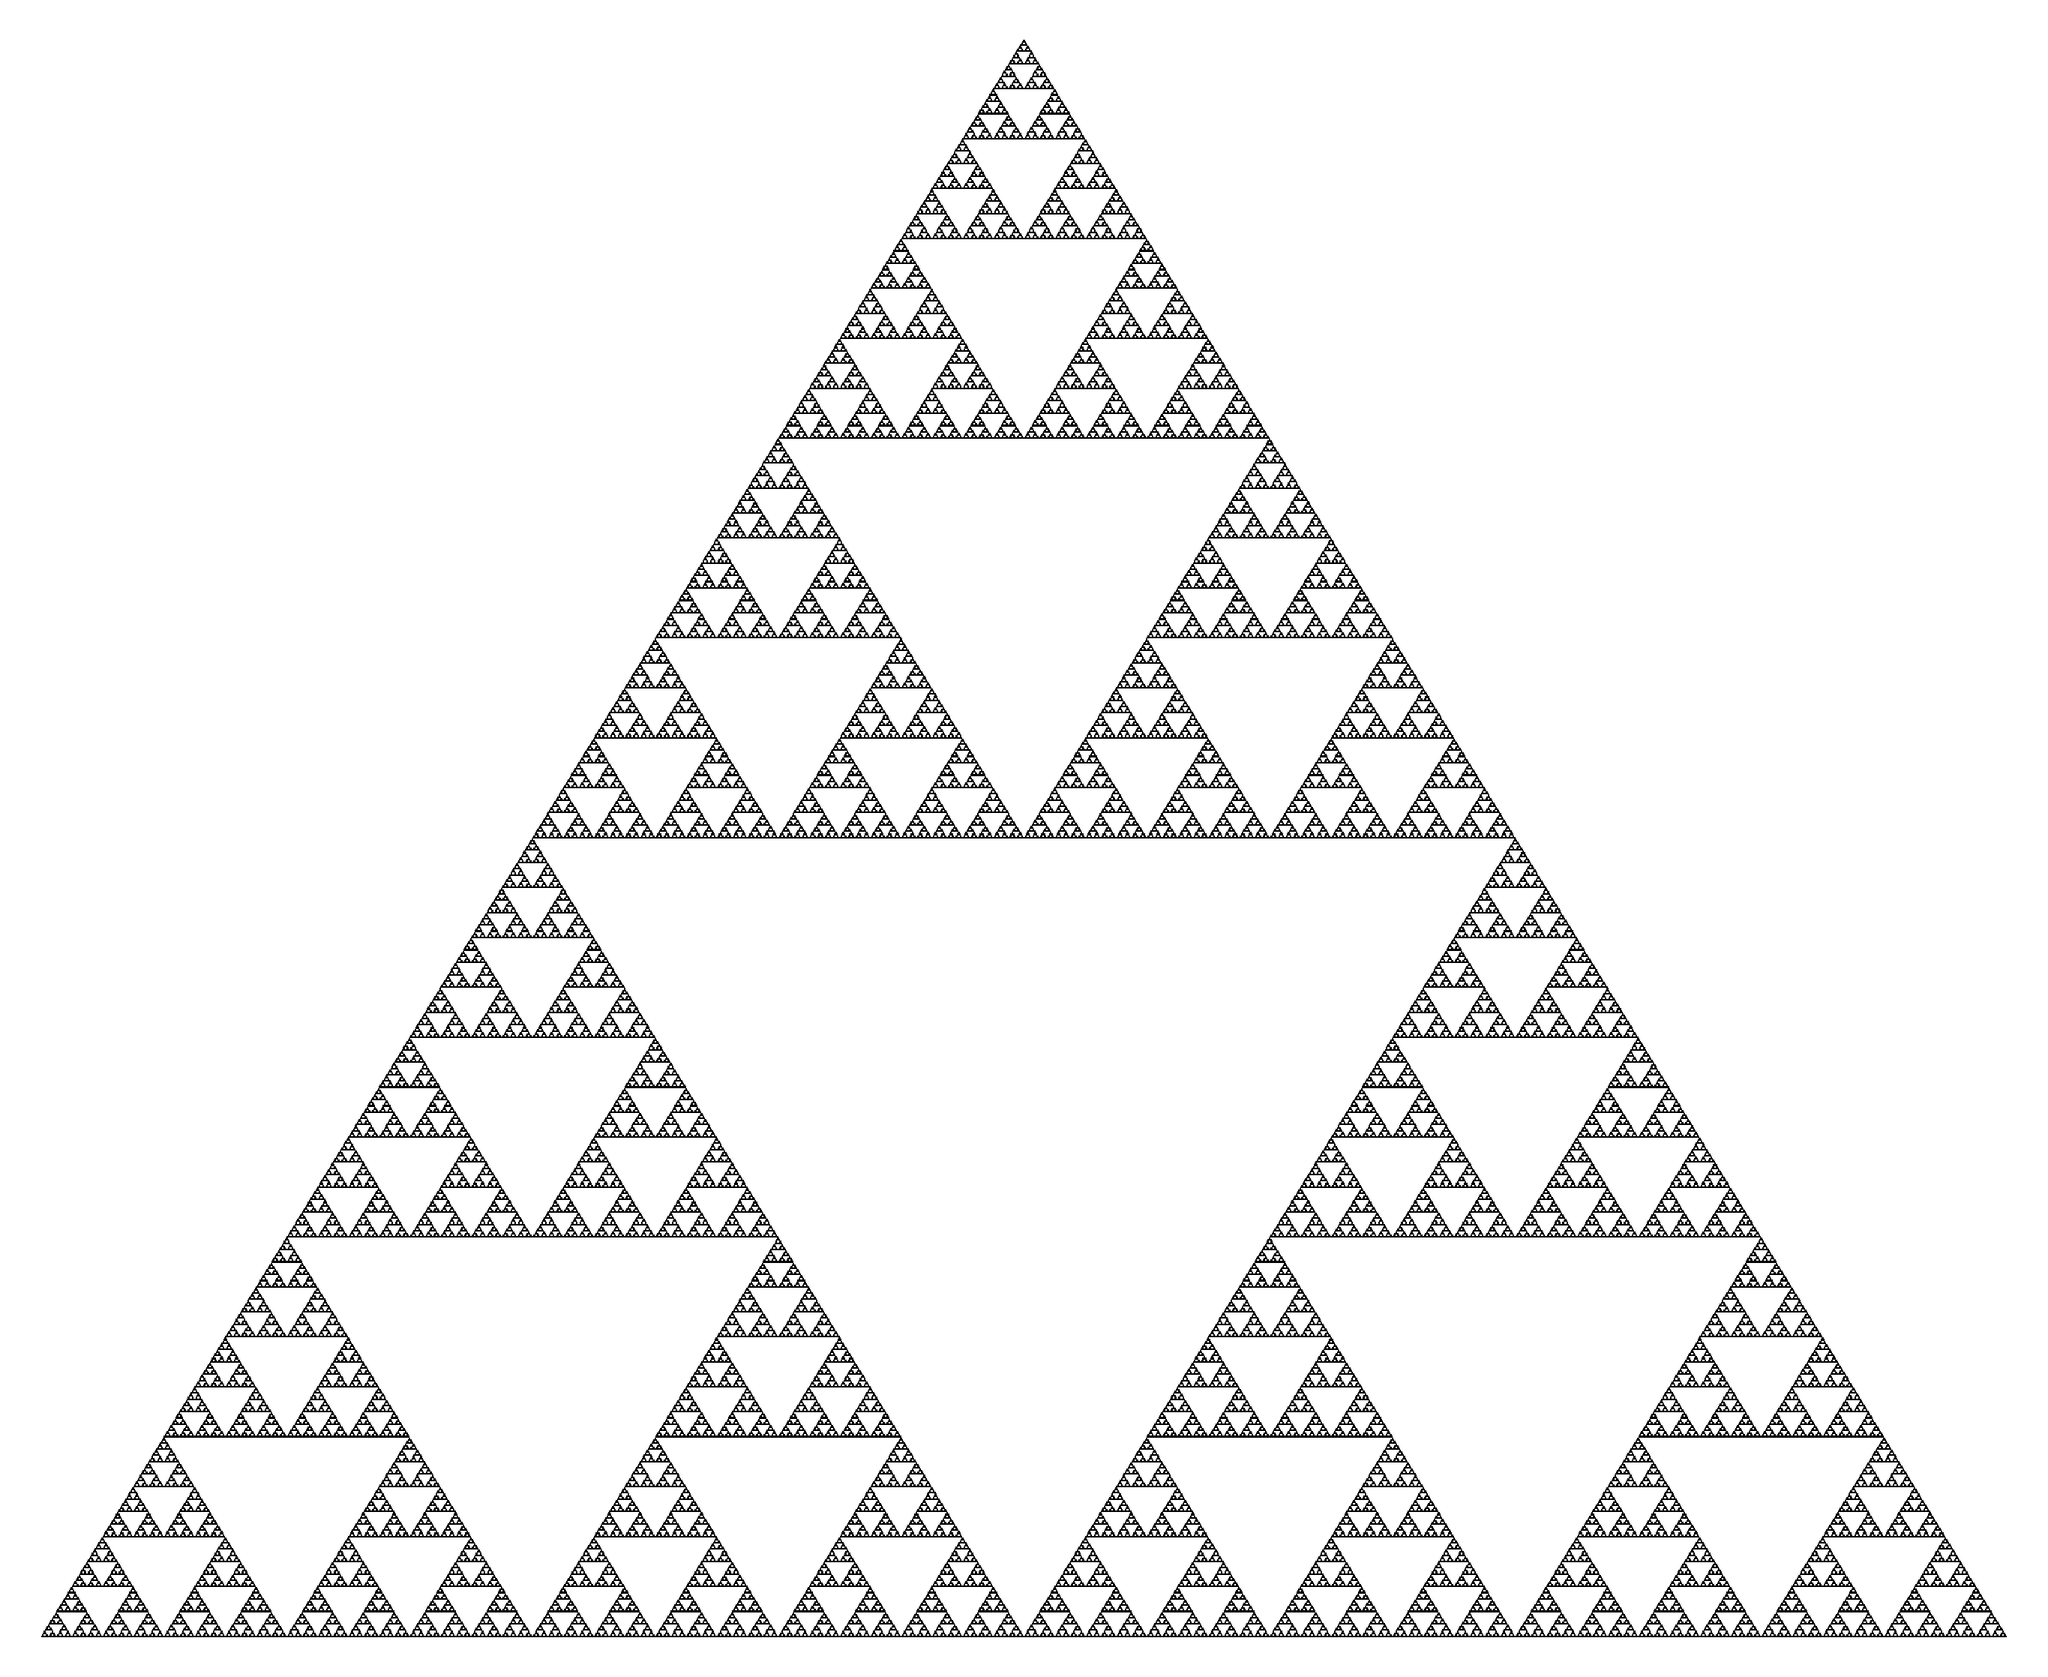
\includegraphics{images/pascal.png}

    \note{I've put this here just because I think it's so cool! See the worksheet zip file for images/pascal.png, which shows the first 1024 rows of Pascal's triangle colored this way.}

    \emph{Just for fun!} Instead of writing down the coefficients of Pascal's triangle, do the following: if the coefficient is odd, color the corresponding hexagon black; otherwise, leave it blank.

    {
      \newdimen\R
      \R=.25cm
      \pgfmathdeclarefunction{coeff}{2}{\binomialCoefficient{#1}{#2}}
      \newcommand\mycolor{white}
      \begin{tikzpicture}[line width=.8pt]
        \foreach \k in {0,...,7}{
          \begin{scope}[shift={(-60:{sqrt(3)*\R*\k})}]
            \pgfmathtruncatemacro\ystart{7-\k}
            \foreach \n in {0,...,\ystart}{
              \pgfmathtruncatemacro\newn{\n+\k}
              \pgfmathsetmacro\binom{factorial(\newn)/(factorial(\k)*factorial(\n))}
              \solonly{\ifthenelse{\isodd{\binom}}{\def\mycolor{black}}{}}
              \begin{scope}[shift={(-120:{sqrt(3)*\R*\n})}]
                \draw[draw=black!30!white, fill=\mycolor] 
                (30:\R) \foreach \x in {90,150,...,330} {
                  -- (\x:\R)}
                -- cycle (90:0)
                node {
                };
              \end{scope}
            }
          \end{scope}
        }
      \end{tikzpicture}
    }

  \end{enumerate}  

\item 

  \note{When we go over this, I will highlight that the terms in $(x + h)^4$ that have $h$ raised to a power $\geq 2$ end up being un-important.}

  \begin{problem}[\vfill]
    Use the definition of the derivative to find
    $\displaystyle\frac{d}{dx} \left(x^4 \right)$.  (In other words, if
    $f(x) = x^4$, find $f'(x)$.) 
  \end{problem}

  \begin{solution} 
    \begin{align*} 
      \displaystyle\frac{d}{dx}(x^4)& =\displaystyle \lim_{h \rightarrow 0 } \frac{ f(x+h) -f(x) }{h} \\
      & = \lim_{h \rightarrow 0} \frac{ (x+h)^4 - x^4}{h} \\ 
      & = \lim_{h \rightarrow 0} \frac{ x^4 +4x^3h+6x^2h^2+4xh^3+h^4 - x^4} {h} \\
      & = \lim_{h \rightarrow 0 } \frac{ 4x^3h+6x^2h^2+4xh^3+h^4}{h} \\
      &= \lim_{h \to 0} \frac{ h(4x^3 + 6x^2 h + 4x h^2 + h^3)}{h} \\
      & = \lim_{h \rightarrow 0 } 4x^3 +6x^2h+4xh^2+h^3 \\ 
      & = 4x^3
    \end{align*}
  \end{solution}  

\item  \label{power-rule}

  \note{We'll do this together. The key thing to recognize is that we can write $(x + h)^n = x^n + n x^{n-1} h + h^2 (\text{stuff})$.}

  \begin{problem}[\vfill]
    If $n$ is any positive integer, use the limit definition of the
    derivative to find $\displaystyle\frac{d}{dx} \left(x^n \right)$.
  \end{problem}

  \begin{solution}
    We can write
    \begin{align*}
      (x + h)^n &= x^n + n x^{n - 1} h + \text{terms that involve $h$ raised to a power $\geq 2$} \\
      \intertext{We can factor $h^2$ out of the terms that involve $h$ raised to a power $\geq 2$, so the previous line can be written}
      &= x^n + n x^{n - 1} h + \bigstar h^2 
    \end{align*}
    where $\bigstar$ is a bunch of stuff we actually don't need to know.
    Then,
    \begin{align*} 
      \displaystyle\frac{d}{dx}(x^n)
      & = \lim_{h \rightarrow 0} \frac{ (x+h)^n - x^n}{h} \\
      & = \lim_{h \rightarrow 0} \frac{ x^n +nx^{n-1}h+ \bigstar h^2 - x^n} {h} \\
      & = \lim_{h \rightarrow 0 } \frac{nx^{n-1}h+\bigstar h^2}{h} \\
      & = \lim_{h \rightarrow 0 } nx^{n-1} + \bigstar h \\
      & = nx^{n-1}
    \end{align*}
  \end{solution}

\item 
  \begin{problem}[\nstretch{0.5}]
    Do the derivatives of $x^{-1}$ and $x^{-2}$ fit the rule you came up with in \ref{power-rule}? How about the derivative of $x^0$?
  \end{problem}

  \begin{solution}
    We know that $\frac{d}{dx}x^{-1}=-x^{-2}$, and
    $\frac{d}{dx}x^{-2}=-2x^{-3}$. Both fit the rule 
    $\frac{d}{dx}x^n = nx^{n-1}$.  The function $x^0$ is
    just the constant function $1$, so we know $\frac{d}{dx}x^0 = 0$.
    This also fits the rule.
  \end{solution}

\end{enumerate}
\begin{framed}
  \textbf{Power Rule:} $\dfrac{d}{dx} \left( x^n \right) = \solonly{nx^{n-1}}$

  \emph{The Power Rule is true for all $n$, including negative values and non-integer values like $-0.5$ and $\pi$, but we've only explained why for positive integers $n$. Nonetheless, you may use it for all $n$.}
\end{framed}

\begin{enumerate}[resume, topsep=0pt]
\item  \label{derivative-rules-gatorade}

  \note{This problem explains the Sum Rule and Constant Multiple Rule.} 

  \raisebox{2ex-\height}{\parbox[t]{1.6in}{
      \vspace{0pt}
      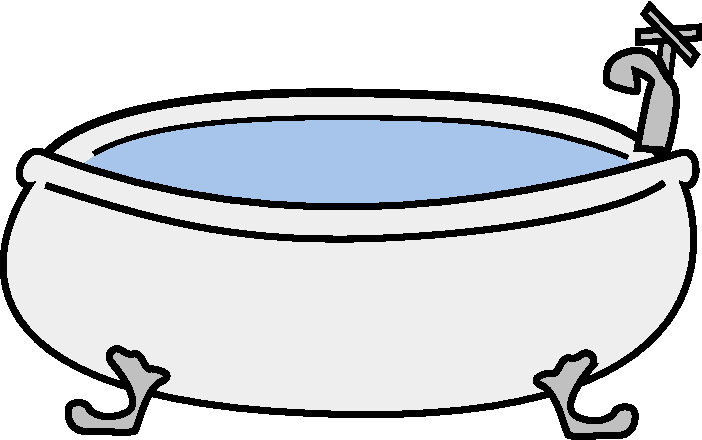
\includegraphics[width=1.5in]{images/bathtub1}
    }
  }
  \begin{minipage}[t]{1.0\linewidth-1.7in}
    At noon one day, Becky and Gregg start making a special blend of purple Gatorade in Becky's bathtub. Let $f(t)$ be the volume (in liters) of blue Gatorade Becky has poured into the tub $t$ minutes after noon, and let $g(t)$ be the volume in liters of red Gatorade Gregg has poured in $t$ minutes after noon.
  \end{minipage}
  \begin{enumerate}
  \item
    \begin{problem}[\stretch{0.5}]
      What does $f + g$ represent? 
    \end{problem}

    \begin{solution}
      $f(t)+g(t)$ is the total volume of Gatorade that Becky and Gregg have
      poured into the bathtub at time $t$.
    \end{solution}

  \item
    \begin{problem}[\vfill]
      What does $(f + g)'$ represent?  What are its units?  How does it
      relate to $f'$ and $g'$? 
    \end{problem}

    \begin{solution}
      $(f+g)'$ represents the rate of change of the volume of Gatorade in the bathtub
      with respect to time. It has units of liters per minute. Since $f'$ is the rate of
      change of the volume of blue Gatorade with respect to time, and $g'$ is the
      rate of change of the volume of red Gatorade with respect to time, it would make
      sense that $(f+g)' = f' + g'$.
    \end{solution}

  \item
    \begin{problem}[\stretch{0.5}]
      Let $h(t)$ be the amount in \uline{gallons} of blue Gatorade that Becky has poured in $t$ minutes after noon. Write an expression for $h(t)$ in terms of $f(t)$. (There are 0.26 gallons in a liter.)
    \end{problem}

    \begin{solution}
      $h(t) = 0.26 f(t)$. 
    \end{solution}

  \item
    \begin{problem}[\vfill]
      What are the units of $h'(t)$?  How does $h'(t)$ relate to $f'(t)$? 
    \end{problem}

    \begin{solution}
      The units of $h'(t)$ would be gallons per minute. It would make sense that
      $h'(t) = 0.26 f'(t)$. 
    \end{solution}

  \end{enumerate}

\end{enumerate}
\begin{framed}
  \textbf{Sum Rule:} $\displaystyle \frac{d}{dx} [f(x) + g(x)] = \probonly{}\solonly{\bm{f'(x) +g'(x)}}$

  \textbf{Constant Multiple Rule:} If $c$ is a constant, then $\displaystyle \frac{d}{dx} [c f(x)] = \probonly{}\solonly{\bm{c f'(x)}}$
\end{framed}

\begin{enumerate}[resume]
\item  \label{differentiation-practice-1}

  \emph{Practice!} Use our new rules to find the derivatives of the following functions. 
  \begin{enumerate}
  \item \label{deriv-of-x^5+5x^4+7}
    \begin{problem}[0.15in]
      $g(x) = x^5 + 5x^4 + 7$
    \end{problem}

    \begin{solution}
      First, since $g(x)$ is a sum of three functions, we can use the Sum Rule.
      \begin{align*}
          \frac{d}{dx} g(x) &= \frac{d}{dx} (x^5 + 5x^4 + 7) \\
          &= \frac{d}{dx} x^5 + \frac{d}{dx} (5x^4) + \frac{d}{dx} 7 \\
          \intertext{Since $5x^4$ is a constant multiple of $x^4$, we can use the Constant
          Multiple Rule.}
          &= \frac{d}{dx} x^5 + 5\frac{d}{dx} x^4 + \frac{d}{dx} 7 \\
          \intertext{Now we can use the Power Rule and fact that the
          derivative of a constant is zero.}
          &= 5x^4 + 5(4x^3) + 0 \\
          &= 5x^4 + 20x^3.
      \end{align*}
    \end{solution}

  \item

    \note{In this and the next part, students need to first rewrite the function so that they can differentiate it. This is a good chance for them to practice working with exponents.

    It's tempting for students to rewrite $\dfrac{1}{4x}$ as $4x^{-1}$ and to think that the derivative of $\pi^6$ is $6 \pi^5$.} 

    \begin{problem}[0.3in]
      $g(x) = \dfrac{5}{\sqrt[3]{x}} - \dfrac{1}{4x} + \sqrt{x^5} + \pi^6$
    \end{problem}

      \begin{solution}
      We can anticipate that we might need to use the Power Rule,
      so let's try to rewrite each term in $g(x)$ to look like $cx^n$.
      Remember that $\pi^6$ is a constant, not a variable.
      \begin{align*}
        g(x) = 5x^{-1/3} -\tfrac{1}{4}x^{-1} + x^{5/2} + \pi^6
      \end{align*}
      We can start by using the Sum Rule.
      \begin{align*}
        \frac{d}{dx} g(x) &= \frac{d}{dx} (5x^{-1/3} -\tfrac{1}{4}x^{-1} + x^{5/2} + \pi^6) \\
        &= \frac{d}{dx}(5x^{-1/3}) + \frac{d}{dx}
        (-\tfrac{1}{4}x^{-1}) + \frac{d}{dx} x^{5/2} + \frac{d}{dx} \pi^6 \\
        \intertext{Now we can use the Constant Multiple Rule.}
        &= 5 \frac{d}{dx}x^{-1/3} + (-\tfrac{1}{4}) \frac{d}{dx}
        x^{-1} + \frac{d}{dx} x^{5/2} + \frac{d}{dx} \pi^6 \\
        &= 5 \frac{d}{dx}x^{-1/3} - \tfrac{1}{4} \frac{d}{dx}
        x^{-1} + \frac{d}{dx} x^{5/2} + \frac{d}{dx} \pi^6 \\
        \intertext{Now we can use the Power Rule.}
        &= 5(-\tfrac{1}{3}x^{-4/3}) -\tfrac{1}{4}(-x^{-2}) + \tfrac{5}{2}x^{3/2} + 0 \\
        &= -\tfrac{5}{3} x^{-4/3} + \tfrac{1}{4} x^{-2} + \tfrac{5}{2} x^{3/2}.
      \end{align*}
    \end{solution}

  \item \label{deriv-of-(x^2-1)/sqrt(x)}
    \begin{problem}[0.3in]
      $h(x) = \dfrac{x^2 - 1}{\sqrt{x}}$
    \end{problem}

    \begin{solution}
      Again, we should try to rewrite $h(x)$ as the sum of terms that look like $cx^n$.
      \begin{align*}
        h(x) &= \frac{x^2-1}{\sqrt{x}} \\
        &= \frac{x^2-1}{x^{1/2}} \\
        &= \frac{x^2}{x^{1/2}} + \frac{-1}{x^{1/2}} \\
        &= x^{3/2} - x^{-1/2}. 
      \end{align*}
      Now we can use the Sum/Difference Rule and the Power Rule.
      \begin{align*}
        \frac{d}{dx} h(x) &= \frac{d}{dx} (x^{3/2} - x^{-1/2}) \\
        &= \frac{d}{dx} x^{3/2} - \frac{d}{dx} x^{-1/2} \\
        &= \tfrac{3}{2} x^{1/2} - (-\tfrac{1}{2}x^{-3/2}) \\
        &= \tfrac{3}{2} x^{1/2} + \tfrac{1}{2}x^{-3/2}
      \end{align*}
    \end{solution}



  \end{enumerate}

  \pspace{\newpage}

\item 

  \note{This is just to make explicit that, once we've calculated $h'(x)$, we can just plug into that to find $h'(\text{any value of interest})$.}

  \begin{problem}[0.75in]
    What's the slope of the line tangent to $y = \dfrac{x^2 - 1}{\sqrt{x}}$ (the function in \ref{deriv-of-(x^2-1)/sqrt(x)}) at $x = 4$? 
  \end{problem}

  \begin{solution}
    The slope of the line tangent to $y=h(x)$ at $x=4$ is $h'(4)$. We can use the
    formula we just found for $h'(x)$.
    \begin{align*}
      h'(4) &= \tfrac{3}{2} (4^{1/2}) + \tfrac{1}{2}(4^{-3/2}) \\
      &= \tfrac{3}{2} (2) + \tfrac{1}{2}(\tfrac{1}{8}) \\
      &= 3 + \tfrac{1}{16} \\
      &= \tfrac{49}{16}
    \end{align*}
  \end{solution}

\item  Let $g(x) = x^5 + 5x^4 + 7$ (the same function as in \ref{deriv-of-x^5+5x^4+7}). 

  \begin{enumerate}

  \item
    \begin{problem}[\vfill]
      On what intervals is $g(x)$ increasing?  On what intervals is it
      decreasing? What are its turning points? 
    \end{problem}

    \begin{solution}
      To determine where $g$ is increasing and decreasing, we should construct a 
      sign chart for $g'(x)$. We determined that $g'(x) = 5x^4 + 20x^3$. 
      
      The first step
      in creating a sign chart for $g'(x)$ is to find the $x$-values for which $g'(x)$ is
      zero or undefined. There are no $x$-values for which $g'(x)$ is undefined. We can
      set $g'(x)$ equal to zero and solve for $x$.
      \begin{align*}
          5x^4 + 20x^3 = 0 \\
          5x^3(x+4) = 0 \\
          x=0 \text{ or } x=-4
      \end{align*}
      This means that we should have the $x$-values $0$ and $-4$ labeled on our sign chart.
      We can plug in $x$-values in various intervals to determine the sign of $g'(x)$. 
      \begin{center}
        \begin{tikzpicture}[scale=0.8]
          \draw[<->] (-3,0) -- (3, 0);
          \node[left] at (-3,0) {$g'(x)$};
          \draw[shift={(-1,0)},color=black] (0pt,3pt) -- (0pt,-3pt) node[below] {$-4$};
          \node[circle, fill=black, inner sep=2pt] at (-1,0) {};
          \draw[shift={(1,0)},color=black] (0pt,3pt) -- (0pt,-3pt) node[below] {$0$};
          \node[circle, fill=black, inner sep=2pt] at (1,0) {};
          \node[above] at (-2,0) {$+$};
          \node[above] at (0,0) {$-$};
          \node[above] at (2,0) {$+$};
        \end{tikzpicture}
      \end{center}

      Based on the sign chart, we can say that
      \begin{itemize}
          \item $g$ is increasing on $(-\infty, -4)$ and $(0, \infty)$ because
          $g'(x)$ is positive on those intervals.
          \item $g$ is decreasing on $(-4, 0)$ because $g'(x)$ is negative on those intervals.
          \item $g$ has turning points at $x=-4$ and $x=0$, because $g'$ changes sign there.
      \end{itemize}
    \end{solution}

  \item

    \note{It's okay to say that $g$ is concave up on $(-3, 0)$ and $(0, \infty)$, or just to say that it's concave up on $(-3, \infty)$. In general, we won't be picky about this.}

    \begin{problem}[\vfill]
      On what intervals is $g(x)$ concave up? On what intervals is it concave down? What are its inflection points?
    \end{problem}

    \begin{solution}
      To determine the intervals on which $g$ is concave up and concave down, we should
      construct a sign chart for $g''(x)$. First, we'll need to find $g''(x)$ by taking
      the derivative of $g'(x)$. 
      \begin{align*}
        \frac{d}{dx} g'(x) &= \frac{d}{dx} (5x^4 + 20x^3) \\
        &= 5\frac{d}{dx}x^4 + 20 \frac{d}{dx}x^3 \\
        &= 20x^3 + 60x^2
      \end{align*}
      Now that we know that $g''(x)=20x^3+60x^2$, we can go ahead and determine the
      $x$-values for which it is undefined or zero. It is never undefined.
      \begin{align*}
        20x^3 + 60x^2 &= 0 \\
        20x^2(x+3) &= 0 \\
        x = 0 \text{ or } x=-3
      \end{align*}
      This means that we should have the $x$-values $-3$ and $0$ on our sign chart. We can
      plug in $x$-values in various intervals to determine the sign of $g''(x)$.
      \begin{center}
        \begin{tikzpicture}[scale=0.8]
          \draw[<->] (-3,0) -- (3, 0);
          \node[left] at (-3,0) {$g''(x)$};
          \draw[shift={(-1,0)},color=black] (0pt,3pt) -- (0pt,-3pt) node[below] {$-3$};
          \node[circle, fill=black, inner sep=2pt] at (-1,0) {};
          \draw[shift={(1,0)},color=black] (0pt,3pt) -- (0pt,-3pt) node[below] {$0$};
          \node[circle, fill=black, inner sep=2pt] at (1,0) {};
          \node[above] at (-2,0) {$-$};
          \node[above] at (0,0) {$+$};
          \node[above] at (2,0) {$+$};
        \end{tikzpicture}
      \end{center}

      Based on the sign chart, we can say that
      \begin{itemize}
          \item $g$ is concave up on on $(-3, \infty)$. It would also be acceptable to say
          $(-3, 0) \cup (0, \infty)$. This is because $g''(x)$ is positive on those intervals.
          \item $g$ is concave down on $(-\infty, -3)$ because $g''(x)$ is negative on that
          interval.
          \item $g$ has an inflection point at $x=-3$ because $g';$ changes sign there.
      \end{itemize}
      
    \end{solution}

  \item

    \note{Obviously, we don't expect them to be able to find the $x$-intercepts. But I'll mention that, when it's easy to do so, it's a good thing to do.}

    \begin{problem}[0.25in]
      What is the $y$-intercept of the graph of $g$? Is it easy to find the $x$-intercepts?
    \end{problem}

    \begin{solution}
      The $y$-intercept is $g(0)$, and $g(0)=7$. To find the $x$-intercepts, we could
      solve the equation $x^5+5x^4+7=0$ for $x$, but this equation is difficult to solve
      by hand.
    \end{solution}

  \item

    \begin{problem}
      What's $\displaystyle \lim_{x \to \infty} g(x)$? \hspace{1in} $\displaystyle \lim_{x \to -\infty} g(x)$?
    \end{problem}

    \begin{solution}
      As $x \to \pm \infty$, the dominant term in $g(x)=x^5 + 5x^4 + 7$ is $x^5$. This means
      that $\displaystyle \lim_{x\to \infty} g(x) = \lim_{x\to \infty} x^5 = \infty$, and 
      $\displaystyle \lim_{x \to -\infty} g(x) = \lim_{x \to -\infty} x^5 = -\infty$.  
    \end{solution}

  \item
    \begin{problem}[\vfill\newpage]
      Sketch a rough graph of $g(x)$ on $[-6, 6]$.  (Note: $g(-6) = -1289$
      and $g(6) = 14263$.)
    \end{problem}

    \begin{solution}
    We know that $g$ should be increasing on $(-\infty, -4)$ and $(0, \infty)$ and 
    decreasing on $(-4, 0)$. We also know that $g$ should be concave down on $(-\infty, -3)$
    and concave up on $(-3, \infty)$. So the graph should look like this.
      \begin{center}
        \begin{tikzpicture}
          \begin{axis}[ytick=\empty]
            \addplot[domain=-5.5:3] {x^5 + 5*x^4 + 7};
          \end{axis}
        \end{tikzpicture}
      \end{center}
    \end{solution}

  \end{enumerate}

\item  \emph{More practice!} Evaluate the derivative of each of the following functions, and simplify your answers. There's one function that you won't be able to differentiate using the rules we've learned so far; which one is it?

  \begin{enumerate}

  \item
    \begin{problem}[\vfill]
      $f(x) = (x^5 - 3x^2 -4) \sqrt[3]{x^2}$
    \end{problem}    

    \begin{solution}
      We should first try to rewrite this $f(x)$ as a sum of terms, where each term
      is a multiple of a power of $x$.
      \begin{align*}
        (x^5 - 3x^2 -4)\sqrt[3]{x^2} &= (x^5 - 3x^2 - 4)(x^{2/3}) \\
        &= x^{17/3} - 3x^{8/3} -4x^{2/3}
        \intertext{Now we can take the derivative using the rules we've learned.}
        f'(x) &= \frac{d}{dx} (x^{17/3} - 3x^{8/3} -4x^{2/3}) \\
        &= \frac{d}{dx} x^{17/3} -3 \frac{d}{dx} x^{8/3} -4\frac{d}{dx} x^{2/3} \\
        &= \tfrac{17}{3} x^{14/3} -3(\tfrac{8}{3}x^{5/3}) -4(\tfrac{2}{3}x^{-1/3}) \\
        &= \tfrac{17}{3} x^{14/3} -8x^{5/3} -\tfrac{8}{3}x^{-1/3} \\
        \intertext{We can simplify by factoring out $\frac{1}{3}x^{-1/3}$.}
        &= \tfrac{1}{3}(x^{-1/3})(17x^{15/3} - 24x^{6/3} -8) \\
        &= \dfrac{17x^5 - 24x^2 -8}{3x^{1/3}}
      \end{align*}
    \end{solution}

  \item
    \begin{problem}[\vfill]
      $r(x) = \sqrt{x^5 - 3x^2 - 4}$
    \end{problem}

    \begin{solution}
      This function can't be rewritten as a sum of multiples of powers of $x$, so we
      can't take its derivative using the rules we've learned so far.
    \end{solution}

  \item
    \begin{problem}[\vfill]
      $f(t) = (t^2 + 1)^2$
    \end{problem}

    \begin{solution}
      We can rewrite this as the sum of multiples of powers of $t$ by expanding.
      \begin{align*}
        (t^2 + 1)^2 &= (t^2 + 1)(t^2 + 1) \\
        &= (t^4 + 2t^2 + 1) \\
        \intertext{Now we can take the derivative using the rules we've learned.}
        f'(t) &= \frac{d}{dt} (t^4 + 2t^2 + 1) \\
        &= \frac{d}{dt} t^4 + 2\frac{d}{dt} t^2 + \frac{d}{dt} 1 \\
        &= 4t^3 + 2(2t) + 0 \\
        &= 4t^3 + 4t.
      \end{align*}
    \end{solution}

  \end{enumerate}

\end{enumerate}
\end{document}
